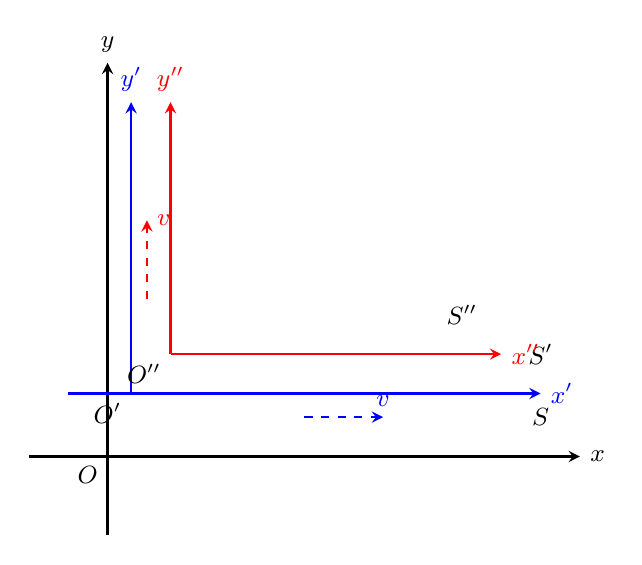
\begin{tikzpicture}[font=\small, >=stealth]
  % 8-30: 三惯性系 S, S', S''
  % S系
  \draw[->, thick] (-1,0) -- (6,0) node[right] {$x$};
  \draw[->, thick] (0,-1) -- (0,5) node[above] {$y$};
  \node at (0,0) [below left] {$O$};
  \node at (5.5,0.5) {$S$};

  % S'系（沿x轴以v运动）
  \draw[->, thick, blue] (-0.5,0.8) -- (5.5,0.8) node[right] {$x'$};
  \draw[->, thick, blue] (0.3,0.8) -- (0.3,4.5) node[above] {$y'$};
  \node at (0.3,0.8) [below left] {$O'$};
  \node at (5.5,1.3) {$S'$};

  % S''系（沿y'轴以v运动）
  \draw[->, thick, red] (0.8,1.3) -- (5,1.3) node[right] {$x''$};
  \draw[->, thick, red] (0.8,1.3) -- (0.8,4.5) node[above] {$y''$};
  \node at (0.8,1.3) [below left] {$O''$};
  \node at (4.5,1.8) {$S''$};

  % 速度标注
  \draw[->, thick, blue, dashed] (2.5,0.5) -- (3.5,0.5) node[above] {$v$};
  \draw[->, thick, red, dashed] (0.5,2) -- (0.5,3) node[right] {$v$};
\end{tikzpicture}
